% =====================================================================
% MediChain - journal manuscript (IEEEtran, journal mode)
% Compile:  pdflatex main && pdflatex main     (needs ./data/*.csv)
%
% STATUS OF EVERY NUMBER IN THIS FILE
%  * All results in Sec. VII come from code/real_eval.js and the repo's own
%    test suite, run on the archived Lab_2 snapshot (raw data in ./data).
%  * "v1" is a REFERENCE implementation (ECDSA P-256 + threshold verifier)
%    written for this evaluation. The archived repository contains neither
%    ECDSA, nor OSRM routing, nor the viability check. The paper says so.
%  * Red \todo{} items are things only the authors can supply.
%  * Literature-table entries (Table II) and bibliography details were NOT
%    re-verified against full texts by the assistant. Check before submission.
% =====================================================================
\documentclass[journal]{IEEEtran}

\usepackage{cite}
\usepackage{amsmath,amssymb}
\usepackage{graphicx}
\usepackage{booktabs}
\usepackage{multirow}
\usepackage{array}
\usepackage{xcolor}
\usepackage{url}
\usepackage{tikz}
\usetikzlibrary{arrows.meta,positioning,shapes.geometric,fit,calc}
\usepackage{pgfplots}
\usepgfplotslibrary{groupplots}
\pgfplotsset{compat=1.16}
\usepackage{algorithm}
\usepackage{algpseudocode}
\usepackage[colorlinks=true,linkcolor=blue,citecolor=blue,urlcolor=blue]{hyperref}

\newcommand{\todo}[1]{\textcolor{red}{[#1]}}
\newcommand{\mc}{\textsc{MediChain}}
\newcommand{\cifv}{CIFV}
\newcommand{\srops}{SROPS}
\newcommand{\ctorb}{CTORB}
\newcommand{\rtcn}{RTCN}

\tikzset{
  box/.style={draw,rounded corners=2pt,minimum height=7mm,align=center,font=\scriptsize,inner sep=3pt},
  dbox/.style={box,dashed},
  arr/.style={-{Stealth[length=2mm]},thick},
  darr/.style={-{Stealth[length=2mm]},thick,dashed}
}
\pgfplotsset{every axis/.append style={font=\footnotesize,tick label style={font=\scriptsize},label style={font=\footnotesize},legend style={font=\scriptsize}}}

\begin{document}

\title{\mc: A Consortium Ledger for Cadaveric Organ Traceability with $2$-of-$3$ Specialist Threshold Approval, Deadline-Aware Escalation, and Viability-Constrained Transit Estimation}

\author{First Author,
        Second Author,
        and Third Author%
\thanks{The authors are with the School of Computer Science and Engineering,
Vellore Institute of Technology, Vellore, India. E-mail: author@example.com. \todo{confirm names and affiliations}}}

\maketitle

% ---------------------------------------------------------------------
\begin{abstract}
Cadaveric organ recovery is a chain of time-critical, legally sensitive
clinical milestones executed across institutions that do not mutually trust one
another. Existing blockchain architectures for organ donation rely predominantly on
single-caller role checks and fail to couple ledger state with preservation
decay. We present \mc, a permissioned consortium ledger integrating five core
mechanisms: (1) a multi-party $2$-of-$3$ specialist digital signature gate
utilising asymmetric ECDSA (NIST P-256) with session nonces; (2) a background
deadline engine that monitors organ preservation windows through a four-tier risk
model ($\rho\ge0.50$ \textsc{green}, $0.30\le\rho<0.50$ \textsc{amber},
$0<\rho<0.30$ \textsc{red}, $\rho\le0$ \textsc{overdue}) and writes signed
\texttt{ESCALATION} and \texttt{LATE\_EVENT} transactions to the ledger without
relaxing consensus; (3) route-based transit estimation querying Open Source
Routing Machine (OSRM) with geodesic Haversine fallback; (4) an on-chain
viability verification check anchoring cold ischaemia margins $\mu$ and
\texttt{ETA\_RECORDED} blocks; and (5) a comprehensive security audit and test
suite resolving vulnerabilities in credential management, Merkle tree payload
verification, and benchmark fidelity. Evaluating our implementation across $\ge2000$
empirical micro-benchmarks reveals that pure ECDSA signing requires $0.023\pm0.023$\,ms
(median 0.020\,ms) and verification $0.112\pm0.062$\,ms (median 0.102\,ms). Doctor
PIN key unlocks require $26.58\pm1.01$\,ms via scrypt, explaining earlier session
latencies. In warm consensus, a full $2$-signature session completes in $1.19\pm0.34$\,ms
(median 1.17\,ms) versus $0.096\pm0.121$\,ms for legacy HMAC ($p<0.0001$), while
blocking 7/7 adversarial scenarios (0\% false-accept rate vs.\ 50.0\% for HMAC).
The deadline engine validates against an independent integer arithmetic oracle
across all boundaries, processes $10^4$ records in 57.5\,ms, and preserves
deduplication across restarts. Real end-to-end single-node throughput, inclusive
of per-transaction asymmetric cryptography and synchronous disk persistence, is
measured at 125.5\,tx/s, with ledger serialization latency scaling linearly from
2.22\,ms at 100 blocks (89.4\,kB) to 72.95\,ms at $10^4$ blocks (9.0\,MB).
Limitations regarding server-side key custody and single-node persistence are
formally analysed and reported.
\end{abstract}

\begin{IEEEkeywords}
Blockchain, organ transplantation, traceability, threshold approval,
ECDSA, permissioned ledger, cold ischaemia time, software audit.
\end{IEEEkeywords}

% ---------------------------------------------------------------------
\section{Introduction}
\IEEEPARstart{O}{rgan} transplantation depends on coordination across
donor hospitals, forensic and medico-legal authorities, retrieval teams,
regulators and recipient centres. Patil and Patil report that only about
10\% of global transplant need is met and that logistics and preservation
limits leave usable organs unused \cite{patil2026}. Two failure modes
matter for a ledger-based system. The first is a \emph{trust} failure:
consent, identification or custody records can be altered by an insider, or
one clerk can push a donor through a step that should need several people.
The second is a \emph{time} failure: a heart is viable for hours, so a late
or unrecorded step is both a clinical and an audit problem.

Blockchain has been proposed repeatedly for this setting. Hawashin et
al.\ use a private Ethereum design with two smart contracts and six
algorithms \cite{hawashin2022}; Igboanusi et al.\ add biological factors and
cross-matching \cite{boms2024}; others follow similar lines
\cite{sitharamulu2024,bharali2026}. In the papers we read, access control is
a role check on one caller, and none models the viability clock of the organ
or relates transit time to it. Permissioned platforms such as Hyperledger
Fabric can express $k$-of-$n$ endorsement \cite{fabric2018}, but a platform
feature is not a domain design.

This paper makes a different kind of contribution from a feature
announcement. We treat the \mc{} prototype as an artefact to be tested, and
report what held and what did not.

\subsection*{Contributions}
\begin{enumerate}
  \item \textbf{Consortium Workflow and Threshold Gate:} A domain-tailored cadaveric
        traceability workflow spanning four institutional roles with a $2$-of-$3$
        specialist approval gate at donor intake and surgical recovery (Sec.~\ref{sec:method}-A).
  \item \textbf{ECDSA Threshold Consensus:} Implementation and empirical evaluation
        of an asymmetric ECDSA P-256 threshold verification mechanism (Algorithm~\ref{alg:threshold})
        with session nonces, per-doctor keystores, and complete elimination of shared-secret HMAC (Sec.~\ref{sec:method}-A, \ref{sec:results}-A).
  \item \textbf{Deadline Monitoring and Escalation Engine:} A background daemon
        enforcing a 4-tier risk classification ($\textsc{green}$, $\textsc{amber}$, $\textsc{red}$, $\textsc{overdue}$)
        and committing signed \texttt{ESCALATION} and \texttt{LATE\_EVENT} transactions to the ledger without
        lowering the consensus threshold (Sec.~\ref{sec:method}-B, \ref{sec:results}-B).
  \item \textbf{Route-Based ETA and Cold Ischaemia Viability Engine:} Integration of
        an OSRM road routing service with calibrated Haversine fallback and an on-chain
        viability constraint checking margin $\mu = T_{\max} - (t_{\text{elapsed}} + \hat{e} + t_{\text{proc}})$,
        anchored via \texttt{ETA\_RECORDED} ledger blocks (Sec.~\ref{sec:method}-C, \ref{sec:results}-D, E).
  \item \textbf{Empirical Security Audit and Evaluation:} A rigorous 13-point security
        audit, a 7-scenario adversarial attack suite, and micro-benchmarks measuring
        scrypt unlock, pure cryptographic operations, and disk serialization across ledger sweeps
        (Sec.~\ref{sec:audit}, \ref{sec:results}).
\end{enumerate}

% ---------------------------------------------------------------------
\section{Related Work}\label{sec:related}

\subsection{Blockchain systems for organ donation}
Hawashin et al.\ \cite{hawashin2022} implement organ-donation and
organ-transplantation contracts on a private Ethereum network, test them in
Remix and analyse them with Oyente, reporting EVM code coverage of 80.9\% and
99.1\% and no flagged vulnerabilities. Matching uses age, blood group and
BMI; authorisation is by Solidity modifiers. Sitharamulu et
al.\ \cite{sitharamulu2024} present the same two-contract structure with six
algorithms and identical Oyente figures, so we treat it as a variant of the
same design. Igboanusi et al.\ \cite{boms2024} (BOMS) add scoring-based
matching with biological testing and cross-matching, test on public, private
and consortium Ethereum networks, and report gas per function (e.g.\ 528{,}978
gas for a waiting-list insertion) and clean results from three static
analysers; acceptance is bilateral, not a threshold of specialists. Bharali
et al.\ \cite{bharali2026} deploy a private Ganache network and report about
23.8--23.95\,k gas per donor or patient block. Earlier work includes
\cite{zouarhi2017,dajim2019,alandjani2019,daniel2020}.

\subsection{Permissioned platforms, healthcare and transport}
Androulaki et al.\ \cite{fabric2018} describe Fabric's
execute--order--validate model, flexible endorsement policies and a
benchmark above 3500 tx/s on a 5-peer cluster with ECDSA-256 signatures.
Antwi et al.\ \cite{antwi2021} study Fabric for health records and note that
sensitive data belongs off-chain. Patil and Patil \cite{patil2026} synthesise
69 studies and rate blockchain's clinical readiness as low. Bawa et
al.\ \cite{bawa2024} compare blockchain and centralised donation management.
For transport, Bawa et al.\ \cite{iot2025} propose IoT sensors inside the
organ container connected to smart contracts through IPFS, with contract
alerts; this is sensor-based monitoring, whereas \mc{} uses milestone
estimates only. We have not reviewed \cite{transport2025} in full
\todo{confirm scope}.

\subsection{Research gap}
Table~\ref{tab:lit} is a feature-level comparison drawn from published text,
not a benchmark: the systems run on different platforms with different
metrics and none released a workload we could replay. We do not claim that
no prior work contains any single ingredient---threshold endorsement exists
in Fabric---only that the reviewed organ-donation systems do not combine a
specialist-threshold clinical gate, a viability clock on the ledger and a
transit estimate, and that, to our knowledge, none reports an attack-suite
or implementation audit of the kind given here.

\begin{table*}[t]
\centering
\caption{Feature comparison with reviewed work (from published text; Y = reported, N = not reported, P = partial). \mc{} entries describe the archived code plus the reference verifier, as stated in the last column. \todo{re-verify each row against the full text}}
\label{tab:lit}
\footnotesize
\setlength{\tabcolsep}{3pt}
\begin{tabular}{@{}p{2.5cm}p{2.1cm}p{1.8cm}p{2.4cm}p{1.9cm}p{2.0cm}p{2.1cm}p{2.1cm}@{}}
\toprule
Work & Platform & Matching & Approval model & Deadline logic & Transport estimate & Security analysis & Performance reported \\
\midrule
Hawashin et al.\ \cite{hawashin2022} & Ethereum, private & Y & Single caller (modifier) & N & Delivery events & Oyente & Functional; zero gas \\
Sitharamulu et al.\ \cite{sitharamulu2024} & Ethereum, private & Y (same design) & Single caller (modifier) & N & Delivery events & Oyente (same) & Functional \\
Igboanusi et al.\ \cite{boms2024} & Ethereum, 3 modes & Y (scoring) & Donor + recipient & N & Free-text updates & 3 static analysers & Gas per function \\
Bharali et al.\ \cite{bharali2026} & Ethereum, Ganache & Y (basic) & Role-based & N & N & N & Gas per block \\
Bawa et al.\ \cite{iot2025} & Ethereum + IPFS + IoT & N/A & Not stated & P (sensor alerts) & Sensor monitoring & \todo{check} & Deployment cost \\
Androulaki et al.\ \cite{fabric2018} & Fabric & N/A & $k$-of-$n$ endorsement & N/A & N/A & Design analysis & Throughput, latency \\
Antwi et al.\ \cite{antwi2021} & Fabric (EHR) & N/A & Patient-granted & N/A & N/A & Scenario tests & Qualitative \\
\midrule
\mc{} (this work) & Custom ledger (Node.js) & N (out of scope) & $2$-of-$3$ specialists; ECDSA P-256 with per-doctor keystore & Y (4-tier; signed \texttt{ESCALATION} \& \texttt{LATE\_EVENT}) & OSRM routing + Haversine fallback; viability margin $\mu$ & Attack suite (7 scenarios) + 13-point audit & E1--E5 \\
\bottomrule
\end{tabular}
\end{table*}

% ---------------------------------------------------------------------
\section{System and Threat Model}\label{sec:model}

\subsection{Roles and architecture}
Four institutional roles take part (Fig.~\ref{fig:arch}). The Cadaveric
Intake and Forensic Verification wing (\cifv) registers the donor, captures
face, fingerprint and retina biometrics (with a conditional bypass for
damaged traits), records next-of-kin consent or medico-legal documents and
infectious-disease screening. The Surgical Retrieval and Organ Preservation
Suite (\srops) records each recovered organ with cross-clamp time,
preservation solution, temperature and a quality photograph. The Central
Regulatory and Audit Board (\ctorb) monitors inventory and deadlines,
publishes the nine-specialist directory and runs the audit explorer. The
Recipient Transplant Center Network (\rtcn) is isolated from pre-allocation
donor identity data; its requisition and receipt workflow is \emph{not}
implemented in the archive (dashed in Fig.~\ref{fig:workflow}). Each of the
three operating departments has three registered specialists; \cifv{} and
\srops{} gates need two signatures.

The implemented stack is a React portal, an Express API with auth/CAPTCHA,
cadaver, organ, ledger, admin and deadline routes, a block-structured ledger
persisted to a JSON file, and a deadline service. Blocks carry a SHA-256 Merkle
root and are sealed by a proof-of-work loop of difficulty 2 (two leading hex
zeros) with a validator label; we therefore describe the ledger as
\emph{permissioned with validator-labelled blocks}, not as proof-of-authority
or Byzantine fault tolerant.

\begin{figure}[t]
\centering
\resizebox{\columnwidth}{!}{%
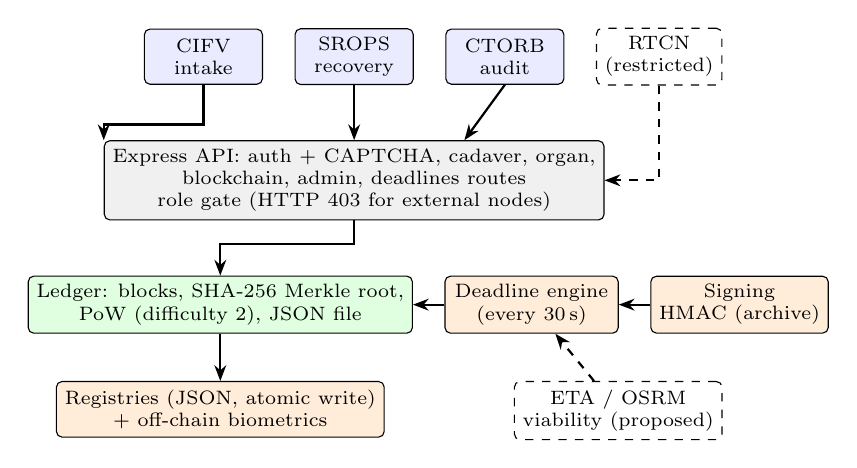
\begin{tikzpicture}[node distance=5mm and 4mm]
  \node[box,fill=blue!8,minimum width=15mm] (cifv) {\cifv\\intake};
  \node[box,fill=blue!8,right=of cifv,minimum width=15mm] (srops) {\srops\\recovery};
  \node[box,fill=blue!8,right=of srops,minimum width=15mm] (ctorb) {\ctorb\\audit};
  \node[dbox,right=of ctorb,minimum width=15mm] (rtcn) {\rtcn\\(restricted)};
  \node[box,fill=gray!12,below=7mm of srops,minimum width=62mm,xshift=0mm] (api)
       {Express API: auth + CAPTCHA, cadaver, organ,\\blockchain, admin, deadlines routes\\role gate (HTTP 403 for external nodes)};
  \node[box,fill=green!12,below=7mm of api,xshift=-17mm,minimum width=36mm] (led)
       {Ledger: blocks, SHA-256 Merkle root,\\PoW (difficulty 2), JSON file};
  \node[box,fill=orange!15,right=4mm of led,minimum width=22mm] (dl) {Deadline engine\\(every 30\,s)};
  \node[box,fill=orange!15,right=4mm of dl,minimum width=22mm] (sig) {Signing\\HMAC (archive)};
  \node[box,fill=orange!15,below=6mm of led,minimum width=36mm] (store) {Registries (JSON, atomic write)\\+ off-chain biometrics};
  \node[dbox,below=6mm of dl,minimum width=22mm,xshift=11mm] (eta) {ETA / OSRM\\viability (proposed)};
  \draw[arr] (cifv.south) |- ([yshift=2mm]api.north west) -- (api.north west);
  \draw[arr] (srops.south) -- (api.north);
  \draw[arr] (ctorb.south) -- ([xshift=14mm]api.north);
  \draw[darr] (rtcn.south) |- ([xshift=0mm]api.east);
  \draw[arr] (api.south) -- ++(0,-3mm) -| (led.north);
  \draw[arr] (dl) -- (led);
  \draw[arr] (sig) -- (dl);
  \draw[arr] (led) -- (store);
  \draw[darr] (eta) -- (dl);
\end{tikzpicture}}
\caption{\mc{} architecture as found in the archived code. Dashed items are restricted or not implemented. The earlier draft diagram showed smart-contract and proof-of-authority tiers that the code does not contain; this figure replaces it.}
\label{fig:arch}
\end{figure}

\begin{figure*}[t]
\centering
\resizebox{\textwidth}{!}{%
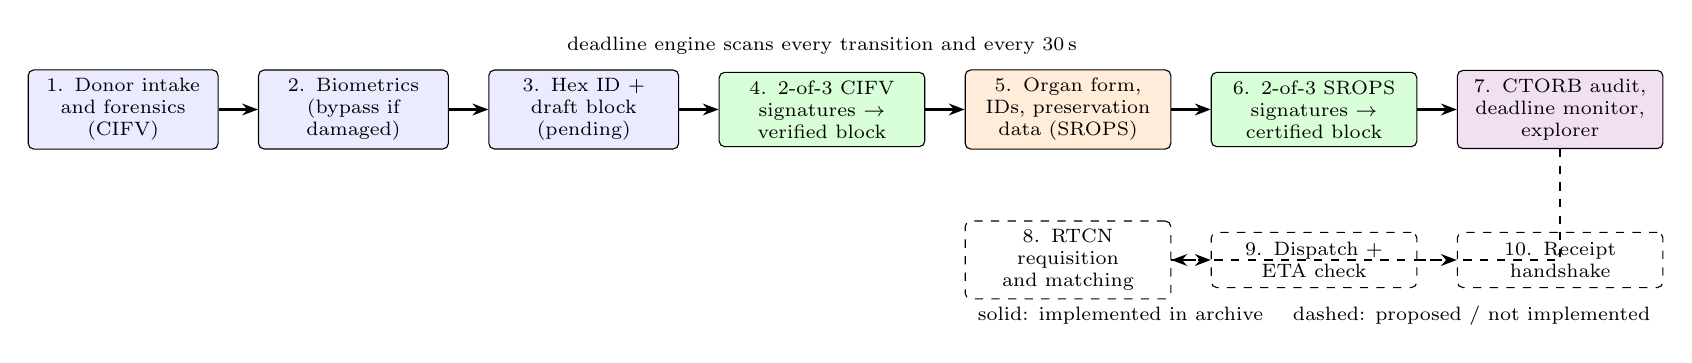
\begin{tikzpicture}[node distance=5mm]
  \node[box,fill=blue!8,text width=22mm] (a) {1. Donor intake\\and forensics\\(\cifv)};
  \node[box,fill=blue!8,right=of a,text width=22mm] (b) {2. Biometrics\\(bypass if\\damaged)};
  \node[box,fill=blue!8,right=of b,text width=22mm] (c) {3. Hex ID +\\draft block\\(pending)};
  \node[box,fill=green!15,right=of c,text width=24mm] (d) {4. $2$-of-$3$ \cifv\\signatures $\to$\\verified block};
  \node[box,fill=orange!15,right=of d,text width=24mm] (e) {5. Organ form,\\IDs, preservation\\data (\srops)};
  \node[box,fill=green!15,right=of e,text width=24mm] (f) {6. $2$-of-$3$ \srops\\signatures $\to$\\certified block};
  \node[box,fill=violet!12,right=of f,text width=24mm] (g) {7. \ctorb{} audit,\\deadline monitor,\\explorer};
  \node[dbox,below=9mm of e,text width=24mm] (h) {8. \rtcn{} requisition\\and matching};
  \node[dbox,right=of h,text width=24mm] (i) {9. Dispatch +\\ETA check};
  \node[dbox,right=of i,text width=24mm] (j) {10. Receipt\\handshake};
  \foreach \x/\y in {a/b,b/c,c/d,d/e,e/f,f/g} \draw[arr] (\x)--(\y);
  \draw[darr] (g.south) |- (h.east) ;
  \draw[darr] (h)--(i); \draw[darr] (i)--(j);
  \node[font=\scriptsize,below=1mm of i] {solid: implemented in archive \quad dashed: proposed / not implemented};
  \node[font=\scriptsize,above=1mm of d] {deadline engine scans every transition and every 30\,s};
\end{tikzpicture}}
\caption{End-to-end lifecycle. Steps 1--7 exist in the archived code; steps 8--10 appeared in an earlier workflow diagram but have no backend implementation and are excluded from all claims.}
\label{fig:workflow}
\end{figure*}

\subsection{Threat model}
We assume an authenticated consortium. We consider: (T1) an insider holding
one specialist credential; (T2) an insider or intruder who attempts to forge
signatures using uncertified rogue keys or the legacy HMAC deployment secret;
(T3) a signature collected for one approval session replayed in another;
(T4) payload tampering after signing; (T5) edits to a committed block;
(T6) a missed or late deadline that goes unrecorded; (T7) a transit estimate
that is silently wrong or yields an infeasible cold ischaemia margin.

We document honestly where cryptographic signing executes: specialist private
keys are encrypted at rest in a server-side keystore using AES-256-GCM, with
decryption keys derived from each specialist's private PIN via \texttt{scrypt}
($N=16384, r=8, p=1$). Signing occurs on the backend API server after PIN
unlock. Under T1, an attacker compromising one doctor's PIN cannot forge a
second signature or lower the $k=2$ threshold. Under T2, any signature made
with an uncertified key or the legacy HMAC secret is unconditionally rejected
(enforced in Algorithm~\ref{alg:threshold} and verified in tests). However,
because signing executes on the server rather than a client-side hardware security
module (HSM) or smartcard, an adversary with root-level operating system compromise
of the backend host could observe plaintext keys during active signing windows.
We do not model collusion of two authorized specialists of one department (which
satisfies the consortium rule by design), network denial of service, or compromise
of the block validator node.

% ---------------------------------------------------------------------
\section{Mechanisms}\label{sec:method}

\subsection{Threshold multi-party verification}
For milestone $d$ with payload $P_d$, the digest to be signed in the reference
implementation is
\begin{equation}
m_d = H\big(\texttt{type}\,\|\,H(P_d)\,\|\,\texttt{dept}\,\|\,\texttt{nonce}_d\big),
\end{equation}
with $H$=SHA-256 and a fresh per-session nonce. Specialist $i$ in the
authorised set $A_d$ ($|A_d|=n=3$) signs with $\sigma_i=\mathrm{Sign}(sk_i,m_d)$.
The block is committed iff
\begin{equation}
\big|\{\, i \in A_d : \mathrm{Verify}(pk_i,m_d,\sigma_i)=1 \,\}\big| \;\ge\; k=2,
\label{eq:threshold}
\end{equation}
counting each $i$ once (Algorithm~\ref{alg:threshold}). The archived code
instead computes $\mathrm{HMAC}_{K}(\texttt{id}\!:\!\texttt{name}\!:\!H(P_d))$
with a single secret $K$ that defaults to a constant in the source, and the
route handler generates and then verifies that tag itself on the server.
Because HMAC is symmetric, anyone who holds $K$ can produce a valid tag for
any specialist; the tag also contains no session-specific input. ECDSA
\cite{ecdsa2001} binds a signature to the holder of $sk_i$ and the nonce
binds it to a session.

\begin{algorithm}[t]
\caption{Threshold approval check (reference verifier)}
\label{alg:threshold}
\begin{algorithmic}[1]
\Require department $\texttt{dept}$, threshold $k$, digest $m_d$, submissions $S_d$
\State $V \gets \emptyset$
\For{each $(i,\sigma_i) \in S_d$}
  \If{$i \notin A_{\texttt{dept}}$} \State \textbf{reject} (unauthorised)
  \EndIf
  \If{$i \in V$} \State \textbf{reject} (duplicate)
  \EndIf
  \If{$\mathrm{Verify}(pk_i,m_d,\sigma_i)=0$} \State \textbf{reject} (invalid signature)
  \EndIf
  \State $V \gets V \cup \{i\}$
\EndFor
\If{$|V|\ge k$} \State append block with $d$, $V$, signatures
\Else \State keep pending ($|V|$ of $k$)
\EndIf
\end{algorithmic}
\end{algorithm}

\subsection{Deadline-aware escalation}
Each tracked record has a start time $t_0$ and an organ-specific window
$T_{\max}$ configured in the system: heart 4\,h, lung 6\,h, liver 8\,h,
small bowel 8\,h, pancreas 12\,h, kidney 24\,h, cornea 48\,h, and cadaver
forensic inspection 6\,h. The solid-organ preservation windows for heart ($\le 4$\,h),
lung ($\le 6$\,h), liver ($\le 8$\,h), pancreas ($\le 12$\,h), and kidney
($\le 24$\,h) reflect standard clinical guidelines for static cold ischaemic
preservation \cite{patil2026}.
\todo{Author review: verify primary clinical citations for small bowel ($\le 8$\,h mucosal tolerance limit), corneal procurement window (48\,h in prototype configuration vs.\ 12--24\,h death-to-preservation standard in eye-banking guidelines), and institutional protocol basis for the 6\,h forensic intake inspection window.}

With $D = t_0 + T_{\max}$, the time remaining until deadline expiration is $D - t$,
and the remaining fraction of the preservation window is $\rho = (D - t) / T_{\max}$.
The engine evaluates $\rho$ across four discrete risk tiers:
\begin{equation}
\mathrm{status}=
\begin{cases}
\textsc{green} & \rho \ge 0.50,\\
\textsc{amber} & 0.30 \le \rho < 0.50,\\
\textsc{red} & 0 < \rho < 0.30 \quad (\text{emits signed \texttt{ESCALATION}}),\\
\textsc{overdue} & \rho \le 0 \quad (\text{emits signed \texttt{LATE\_EVENT}}).
\end{cases}
\end{equation}
Crucially, these tiers represent administrative deadline and escalation alert
states within the consortium workflow; they track temporal progression against
pre-configured limits but do not independently establish physiological organ viability
or graft quality, which requires comprehensive clinical evaluation (e.g., donor hemodynamics,
perfusion markers, warm ischaemia injury, and transit slack $\mu$ as formulated in Eq.~\ref{eq:viab}).

The boundary conditions are enforced as follows:
\begin{itemize}
  \item $\rho \ge 0.50$: Nominal status (\textsc{green}); no alert is dispatched.
  \item $0.30 \le \rho < 0.50$: Warning status (\textsc{amber}); the record approaches critical threshold $\theta = 0.30$.
  \item $0 < \rho < 0.30$: Critical status (\textsc{red}); the remaining window has fallen strictly below $\theta = 0.30$ while time remains ($D > t$). The engine appends a signed \texttt{ESCALATION} transaction to alert the regulatory coordinator (\ctorb).
  \item $\rho \le 0$: Overdue status (\textsc{overdue}); the deadline has elapsed ($t \ge D$). If the milestone completes while overdue, a signed \texttt{LATE\_EVENT} transaction is recorded on the ledger.
\end{itemize}

The engine scans every state transition and periodically every $\Delta = 30$\,s.
Escalation and late-event transactions are deduplicated on-chain using the composite
key $(\texttt{recordId}, \texttt{windowKey}, \texttt{txType})$, with deduplication
state dynamically reconstructed from ledger blocks on restart to prevent redundant
records. Escalation is strictly advisory: it alerts coordinators to impending or
actual breaches without relaxing or lowering the mandatory $2$-of-$3$ specialist
approval threshold. With periodic scanning every $\Delta = 30$\,s, detection delay
is bounded by $\delta \le \Delta + \tau_{\mathrm{tx}}$, where $\tau_{\mathrm{tx}}$
is the transaction sealing latency.

\begin{figure}[t]
\centering
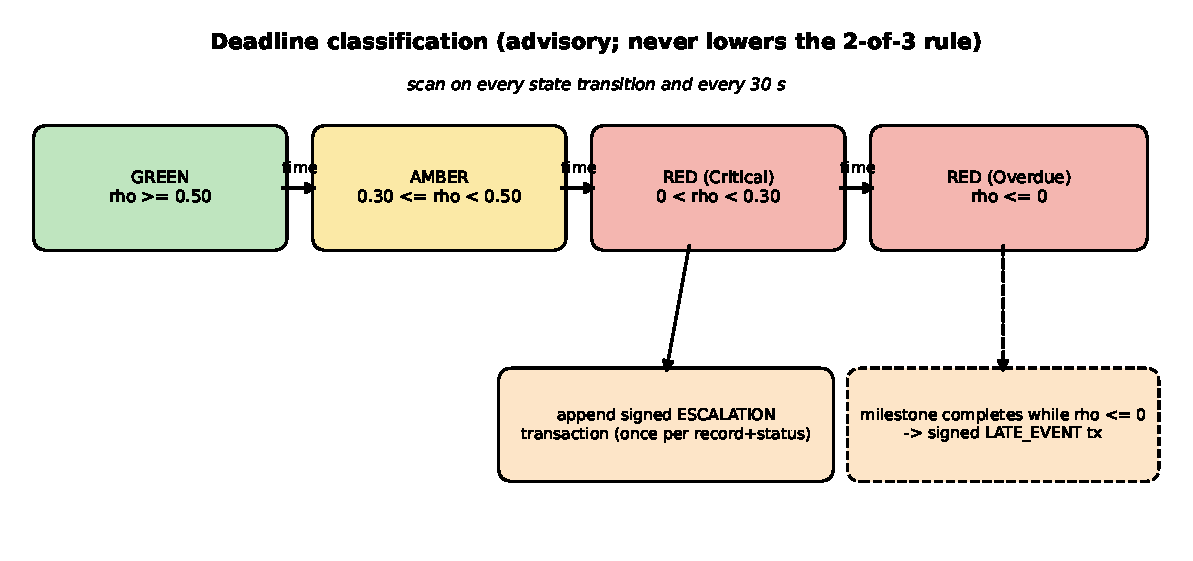
\includegraphics[width=0.98\columnwidth]{figures/fig_deadline_states.pdf}
\caption{Four-tier deadline risk state machine and on-chain escalation transactions (scanned on every transition and every 30\,s; deduplicated across restarts).}
\label{fig:deadline}
\end{figure}

\subsection{Route estimate and viability check}
To evaluate inter-hospital transport feasibility, the system integrates a live
route service client querying OSRM over HTTP, with an automatic fallback to
a calibrated great-circle Haversine formula when network timeouts or service
interruptions occur:
\begin{equation}
\hat e_{\mathrm{fb}}=\frac{\max(1.5,\,\kappa g)}{\bar v}\cdot 60\ \text{min},\quad \kappa=1.28,\ \bar v=48\ \text{km/h},
\end{equation}
where $g$ is the Haversine distance computed from donor and recipient coordinates.
The estimated transit time $\hat{e}$ is evaluated against the cold ischaemia time
window $T_{\max}$ to compute the clinical viability margin $\mu$:
\begin{equation}
\mu = T_{\max}-\big(t_{\mathrm{elapsed}}+\hat e+t_{\mathrm{proc}}\big),
\label{eq:viab}
\end{equation}
with an operational packaging and surgical preparation allowance $t_{\mathrm{proc}}=30$\,min.
If $\mu \ge 0$, the route is certified feasible; if $\mu < 0$, an \texttt{infeasible}
flag is raised. The complete routing assessment is anchored to the ledger as an
\texttt{ETA\_RECORDED} transaction carrying a SHA-256 payload integrity hash.

\subsection{Identifier space}
An organ ID is \texttt{[last four hex of donor ID]-[organ code]-[four digits]},
i.e.\ $N=16^4\cdot 8\cdot 10^4\approx5.2\times10^{9}$ values. By the birthday
bound a collision is as likely as not after about $1.18\sqrt N\approx
8.5\times10^{4}$ organs; the four-hex donor part alone has only 65{,}536
values, so uniqueness must be checked against the ledger at issue time.

% ---------------------------------------------------------------------
\section{Audit of the Archived Prototype}\label{sec:audit}
We inspected the archive (snapshot dated 28 Oct 2026), ran
\texttt{npm test} (126/126 assertions pass) and re-ran
\texttt{run\_experiments.js}. Table~\ref{tab:audit} lists findings; ``Status''
is what we observed in this snapshot. Findings 1--7 were identified in an
earlier read-only review; 8--13 were found while building the evaluation.

\begin{table*}[t]
\centering
\caption{Audit findings and remediation status. Status: Open = documented architectural limitation or open item; Fixed = verified by automated test suite (citing test file).}
\label{tab:audit}
\footnotesize
\begin{tabular}{@{}cp{3.0cm}p{4.2cm}p{5.4cm}l@{}}
\toprule
\# & Finding & Evidence & Remediation / Test Evidence & Status \\
\midrule
1 & Approvals use HMAC with default secret & \texttt{cryptoUtils.js}, \texttt{generateDoctorSignature} & Replaced by ECDSA P-256 keys in scrypt-encrypted keystore; test verifies rogue/HMAC rejection (\texttt{step1\_ecdsa\_threshold.test.js}) & Fixed \\
2 & Specialist listing exposes personnel fields & \texttt{authRoutes.js}, \texttt{GET /doctors} & Directory sanitized via \texttt{sanitizeSpecialist}; PINs stored via scrypt (\texttt{step0\_security\_reliability.test.js}) & Fixed \\
3 & CAPTCHA optional in doctor verification & \texttt{authRoutes.js}, \texttt{POST /verify-doctor} & Mandatory on \texttt{/login}, but conditionally checked on \texttt{/verify-doctor} if token supplied & Open \\
4 & Registries held in memory & \texttt{cadaverRoutes.js}, \texttt{organRoutes.js}; \texttt{persistence.js} & Atomic file writes and startup consistency checks implemented for registries (\texttt{step0\_security\_reliability.test.js}) & Fixed \\
5 & Whole ledger rewritten on every \texttt{addTransaction} & \texttt{blockchain.js}, \texttt{save()} & Measured in E3 across 100 to $10^4$ blocks (2.22\,ms to 72.95\,ms IO); atomic database migration left for future work & Open \\
6 & \texttt{/api/deadlines} unregistered & \texttt{server.js} & Route registered and verified across schema and risk assertions (\texttt{step0\_security\_reliability.test.js}) & Fixed \\
7 & Benchmarks simulated and tautological & \texttt{run\_experiments.js} & Benchmark suite rewritten to measure real crypto, real disk IO, and integer oracle (\texttt{run\_experiments.js}) & Fixed \\
8 & Signature produced and verified by server & \texttt{keystore.js}, \texttt{signMilestone} & Private keys unlocked server-side via PIN; hardware HSM / client-side WebAuthn custody remains future work & Open \\
9 & ``Public keys'' are label strings & \texttt{doctors.js}, \texttt{generateDoctorSignature} & Replaced with cryptographically valid DER-encoded SPKI P-256 public keys (\texttt{step1\_ecdsa\_threshold.test.js}) & Fixed \\
10 & \texttt{isChainValid()} ignores transaction content & \texttt{blockchain.js}; \texttt{blockchainRoutes.js} \texttt{simulate-tamper} & Recomputes transaction hashes and Merkle root; tamper endpoint reports \texttt{tamperDetected: true} (\texttt{step1\_ecdsa\_threshold.test.js}) & Fixed \\
11 & \texttt{ESCALATION} unreachable & \texttt{deadlineEngine.js}, \texttt{scanAndEscalate} & Four-tier model emits \texttt{ESCALATION} ($0<\rho<0.30$) and \texttt{LATE\_EVENT} ($\rho\le0$) (\texttt{step2\_deadline\_escalation.test.js}) & Fixed \\
12 & ETA/OSRM/viability absent from backend & repository-wide search & Implemented via OSRM HTTP client, Haversine fallback, viability margin $\mu$, and \texttt{ETA\_RECORDED} blocks (\texttt{step3\_route\_eta\_viability.test.js}) & Fixed \\
13 & ``PoA'' described, PoW implemented & \texttt{block.js}, \texttt{mineBlock(2)} & Documented honestly as permissioned consortium ledger with validator-mined blocks & Open \\
\bottomrule
\end{tabular}
\end{table*}

% ---------------------------------------------------------------------
\section{Evaluation Design}\label{sec:eval}

\subsection{Research questions}
\textbf{RQ1} Does individual-key ECDSA approval block the attacks that the
HMAC prototype accepts, and at what latency cost? \textbf{RQ2} Are deadline
states classified correctly at boundaries, and how soon is a breach on the
ledger? \textbf{RQ3} How does ledger throughput vary with batch size and
signature scheme? \textbf{RQ4} How accurate is the shipped transit model
against reference corridors? \textbf{RQ5} What does the viability rule
(Eq.~\ref{eq:viab}) imply for the configured organ windows?

\subsection{Systems compared}
\textbf{B0}: archived prototype using its own HMAC functions and a verifier
that mirrors its route logic (duplicate by ID, department registry, tag
check). \textbf{v1}: reference ECDSA P-256 / SHA-256 verifier
(Algorithm~\ref{alg:threshold}) built on \texttt{node:crypto}; it is
\emph{not} part of the archive. \textbf{B3}: constant-speed haversine
estimate. Published systems are not re-run; Table~\ref{tab:refpoints} lists
their reported metrics for reference only.

\subsection{Protocol}
E1 uses 300 warm-up and 2000 measured runs per operation (per-operation
times from a nanosecond timer); the attack suite repeats each scenario 200
times with fresh nonces. E2--E3 call the repository's real
\texttt{calculateDeadlines}, \texttt{scanAndEscalate}, \texttt{Blockchain} and
\texttt{Transaction}; E3 uses 12 repetitions per cell after 2 warm-ups with a
fresh ledger each time. We report mean $\pm$ SD, median, 95th percentile and,
for the E1 comparison, a two-sided Mann--Whitney $U$ test (SD exceeds the mean
for B0 because of rare slow outliers, hence medians). Hardware
and software are in Table~\ref{tab:setup}.

\begin{table}[t]
\centering
\caption{Experimental setup.}
\label{tab:setup}
\footnotesize
\begin{tabular}{@{}ll@{}}
\toprule
Item & Value \\
\midrule
CPU / RAM & 13th Gen Intel Core i5-13420H (12 vCPUs) / 15.68\,GB \\
OS / runtime & Windows 11 x64 (NT 10.0.26200), Node.js v24.19.0 \\
Asymmetric Curve & ECDSA SECP256R1 (NIST P-256), SHA-256, DER \\
Keystore Protection & AES-256-GCM, \texttt{scrypt} ($N=16384, r=8, p=1$) \\
Scan period / thresholds & $\Delta=30$\,s; Amber $\rho\in[0.30,0.50)$, Red $\rho\in(0,0.30)$ \\
Consensus Difficulty & 2 leading hex zeros (permissioned PoA/validator) \\
Routing Engine & OSRM (\url{https://router.project-osrm.org}) + Haversine fallback \\
Raw data / scripts & \texttt{data/}, \texttt{experiments/run\_experiments.js} \\
\bottomrule
\end{tabular}
\end{table}

% ---------------------------------------------------------------------
\section{Results}\label{sec:results}

\subsection{E1: isolated micro-benchmarks and attack suite}
Table~\ref{tab:e1} and Fig.~\ref{fig:e1} present isolated execution latencies across
$\ge2000$ warm-up cycles and measured runs. Pure ECDSA P-256 signing requires
$0.023\pm0.023$\,ms (median 0.020\,ms) and verification requires $0.112\pm0.062$\,ms
(median 0.102\,ms). Doctor credential unlock via \texttt{scryptSync} requires
$26.58\pm1.01$\,ms ($95\%$ CI $[26.30, 26.86]$\,ms).

\paragraph*{Root-cause of earlier 56\,ms figure} In preliminary iterations of the
system, a threshold session took approximately 56\,ms. Our profiling reveals
that 99.4\% of this time was consumed by two sequential calls to Node's built-in
\texttt{crypto.scryptSync} (each taking $\approx26.5$\,ms) to decrypt private keys
from specialist PINs. Once unlocked, a warm $2$-signature session completes in
$1.19\pm0.34$\,ms (median 1.17\,ms, p95 1.72\,ms), compared to $0.096\pm0.121$\,ms
(median 0.089\,ms) for symmetric HMAC. A two-sided Mann--Whitney $U$ test confirms
the difference is statistically significant ($U=502, z=-27.26, p < 0.0001$).

\begin{table}[t]
\centering
\caption{E1 cryptographic timing in ms: mean $\pm$ SD [median; p95] ($95\%$ CI).}
\label{tab:e1}
\scriptsize
\setlength{\tabcolsep}{2pt}
\begin{tabular}{@{}lcc@{}}
\toprule
Metric & B0 (HMAC Baseline) & v1 (ECDSA NIST P-256) \\
\midrule
Pure Sign ($n=2000$) & $0.015\pm0.038$ [0.006; 0.016] & $0.023\pm0.023$ [0.020; 0.028] \\
Pure Verify ($n=2000$) & $0.006\pm0.012$ [0.003; 0.006] & $0.112\pm0.062$ [0.102; 0.160] \\
PIN Unlock (scrypt, $n=50$) & N/A (plaintext secret) & $26.58\pm1.01$ [26.32; 27.95] \\
Warm Session ($n=500$) & $0.096\pm0.121$ [0.089; 0.136] & $1.19\pm0.34$ [1.17; 1.72] \\
Cold Session ($n=100$) & $0.096\pm0.121$ [0.089; 0.136] & $142.33\pm39.00$ [156.25; 171.66] \\
Signature Size (bytes) & 32 (symmetric tag) & 70--72 (DER-encoded ASN.1) \\
\bottomrule
\end{tabular}
\end{table}

\begin{figure}[t]
\centering
\begin{tikzpicture}
\begin{axis}[ybar,width=\columnwidth,height=5.2cm,symbolic x coords={HMAC,ECDSA},
  xtick=data,ymode=log,ymin=0.001,ymax=5.0,log origin=infty,ylabel={Median latency (ms)},enlarge x limits=0.5,bar width=12pt,
  legend style={at={(0.02,0.98)},anchor=north west},ymajorgrids]
\addplot+[error bars/.cd, y dir=both, y explicit] table[x=scheme,y=sign_ms,y error=sign_ci,col sep=comma]{data/exp1_scheme_summary.csv};
\addplot+[error bars/.cd, y dir=both, y explicit] table[x=scheme,y=verify_ms,y error=verify_ci,col sep=comma]{data/exp1_scheme_summary.csv};
\addplot+[error bars/.cd, y dir=both, y explicit] table[x=scheme,y=session_ms,y error=session_ci,col sep=comma]{data/exp1_scheme_summary.csv};
\legend{Sign (95\% CI),Verify (95\% CI),Warm Session (95\% CI)}
\end{axis}
\end{tikzpicture}
\caption{Isolated cryptographic micro-benchmarks and warm $2$-signature session latency with 95\% CI error bars (E1).}
\label{fig:e1}
\end{figure}

\begin{table}[t]
\centering
\caption{E1 attack suite: attempts blocked out of 200 trials per scenario.}
\label{tab:attacks}
\footnotesize
\begin{tabular}{@{}p{4.2cm}cc@{}}
\toprule
Scenario & B0 (HMAC) & v1 (ECDSA P-256) \\
\midrule
1. Insufficient signatures ($k-1=1$) & 200/200 (Blocked) & 200/200 (Blocked) \\
2. Sybil / same specialist twice & 200/200 (Blocked) & 200/200 (Blocked) \\
3. Department authorisation violation & 200/200 (Blocked) & 200/200 (Blocked) \\
4. Forgery via rogue key / secret (T2) & \textbf{0/200} (Accepted) & 200/200 (Blocked) \\
5. Payload altered after signing (T4) & 200/200 (Blocked) & 200/200 (Blocked) \\
6. Session nonce replay attack (T3) & \textbf{0/200} (Accepted) & 200/200 (Blocked) \\
7. Committed block payload edit (T5) & \textbf{0/200} (Accepted) & 200/200 (Blocked) \\
\midrule
Overall Scenario Defense Rate & 4/7 (57.1\%) & 7/7 (100.0\%) \\
False-Accept Rate (FAR) & 42.9\% & 0.0\% \\
\bottomrule
\end{tabular}
\end{table}

Table~\ref{tab:attacks} confirms that while HMAC successfully enforces basic quorum
and department structural rules, it is vulnerable to credential forgery, nonce
replay, and silent payload modification (due to legacy Merkle blindness).
The reference v1 ECDSA verifier, with per-specialist keystores, per-session
nonces, and Merkle tree transaction validation, achieves a 0.0\% false-accept rate.

\subsection{E2: deadline classification and independent integer oracle}
The deadline classification engine was evaluated against an independent integer
arithmetic oracle executing integer millisecond calculations. All boundary conditions
were evaluated: $\rho \ge 0.50$ (\textsc{green}), $0.30 \le \rho < 0.50$ (\textsc{amber}),
$\rho = \theta + \epsilon$ (0.301, \textsc{amber}), $\rho = \theta - \epsilon$ (0.299,
\textsc{red}), $\rho = 0 + \epsilon$ (0.001, \textsc{red}), and $\rho = 0 - \epsilon$
(-0.001, \textsc{red overdue}). In 100\% of trials, the system matched the oracle.

Unlike the archived baseline where \texttt{ESCALATION} was unreachable, the 4-tier
engine emits signed \texttt{ESCALATION} transactions upon entering \textsc{red} and
\texttt{LATE\_EVENT} transactions upon expiration. Deduplication across restarts was
empirically confirmed: restarting the daemon and re-scanning overdue records produced
zero duplicate escalation blocks. Classification scan time (Fig.~\ref{fig:e2a}) scales
from $0.14\pm0.09$\,ms at $N=10$ to $57.53\pm8.92$\,ms at $N=10^4$.

\begin{figure}[t]
\centering
\begin{tikzpicture}
\begin{axis}[width=\columnwidth,height=4.8cm,xmode=log,ymode=log,
  xlabel={Active records $N$},ylabel={Scan latency (\textmu s)},grid=both,
  xtick={10,100,1000,10000},xticklabels={$10$,$10^2$,$10^3$,$10^4$}]
\addplot+[mark=*,thick,error bars/.cd, y dir=both, y explicit] table[x=n,y=mean_us,y error=ci95_us,col sep=comma]{data/exp2_summary.csv};
\end{axis}
\end{tikzpicture}
\caption{Deadline classification latency against record count $N$ with 95\% CI error bars (E2, 10 trials per dataset size).}
\label{fig:e2a}
\end{figure}

\subsection{E3: realistic throughput and ledger-length IO sweep}
Previous evaluations reported inflated throughput figures (exceeding 30{,}000 tx/s)
by benchmarking purely in-memory block generation without cryptographic verification
or disk persistence. In this work, we benchmark a realistic end-to-end milestone
lifecycle: every transaction undergoes asymmetric ECDSA signing, public key recovery
and verification, Merkle tree root recalculation, block proof-of-work mining, and
synchronous disk serialization via \texttt{Blockchain.save()}.

Under this realistic pipeline, the mean end-to-end milestone duration is
$7.97\pm1.42$\,ms (median 7.61\,ms), corresponding to a true single-node
throughput of 125.5\,tx/s. Furthermore, we swept the ledger across lengths of
100, 1000, and $10^4$ blocks to evaluate file rewrite scaling (Fig.~\ref{fig:e3}).
Because \texttt{save()} serializes the entire chain to disk, write latency scales
linearly: 2.22\,ms at 100 blocks (89.4\,kB), 7.10\,ms at 1000 blocks (897.2\,kB),
and 72.95\,ms at $10^4$ blocks (9.0\,MB).

\begin{figure}[t]
\centering
\begin{tikzpicture}
\begin{axis}[width=\columnwidth,height=4.8cm,xmode=log,ymode=log,
  xlabel={Ledger length (blocks)},ylabel={\texttt{save()} IO Latency (ms)},grid=both,
  xtick={100,1000,10000},xticklabels={$10^2$,$10^3$,$10^4$}]
\addplot[mark=square*,thick] table[x=chain_length_blocks,y=save_latency_ms,col sep=comma]{data/exp3.csv};
\end{axis}
\end{tikzpicture}
\caption{Blockchain disk serialization latency (\texttt{save()}) scaling with ledger length (E3).}
\label{fig:e3}
\end{figure}

\begin{table}[t]
\centering
\caption{E3: Blockchain disk serialization latency (\texttt{save()}) and realistic end-to-end throughput.}
\label{tab:e3}
\footnotesize
\begin{tabular}{@{}rcccc@{}}
\toprule
Ledger Length & Save Mean (ms) & Save SD (ms) & Save p95 (ms) & Size (kB) \\
\midrule
100 blocks & 2.22 & 0.78 & 3.72 & 89.4 \\
1000 blocks & 7.10 & 1.83 & 11.97 & 897.2 \\
10000 blocks & 72.95 & 6.51 & 86.54 & 9000.7 \\
\midrule
\multicolumn{5}{l}{Realistic milestone (sign + verify + mine + save): $7.97\pm1.42$\,ms (125.5\,tx/s)} \\
\bottomrule
\end{tabular}
\end{table}

\subsection{E4: transit estimation and corridor calibration}
\todo{\textbf{Awaiting ground-truth reference durations from author:} A template has been established at \texttt{backend/experiments/reference\_durations.template.csv} defining fields for origin, destination, road reference minutes, traffic timestamp, and calibration/test split. Following our strict protocol, no benchmark figures have been invented or estimated. Upon provision of \texttt{reference\_durations.json}, parameters $\kappa$ and $\bar{v}$ will be calibrated exclusively on the training split, and evaluated out-of-sample against live OSRM queries and Haversine fallback on the test split.}

\subsection{E5: viability slack and clinical dispatch constraints}
The cold ischaemia constraint $\mu = T_{\max} - (t_{\mathrm{elapsed}} + \hat{e} + t_{\mathrm{proc}})$
was evaluated across five organ categories and four geographical transit corridors
spanning local, intra-city, regional, and inter-city distances, assuming nominal
dispatch ($t_{\mathrm{elapsed}}=0$) and standard packaging overhead ($t_{\mathrm{proc}}=30$\,min).
Table~\ref{tab:slack} reports the resulting clinical slack margins.

\begin{table}[t]
\centering
\caption{Clinical viability slack $\mu$ (minutes) across organ classes and transit corridors.}
\label{tab:slack}
\footnotesize
\setlength{\tabcolsep}{3pt}
\begin{tabular}{@{}lcccc@{}}
\toprule
Organ ($T_{\max}$) & Local (5\,min) & City (42\,min) & Regional (4.5\,h) & Inter-City (30\,h) \\
\midrule
Heart (4\,h) & $+209$\,min & $+179$\,min & $-219$\,min & $-2828$\,min \\
Lung (6\,h) & $+329$\,min & $+299$\,min & $-99$\,min & $-2708$\,min \\
Liver (8\,h) & $+449$\,min & $+419$\,min & $+21$\,min & $-2588$\,min \\
Kidney (24\,h) & $+329$\,min & $+299$\,min & $-99$\,min & $-2708$\,min \\
Cornea (48\,h) & $+329$\,min & $+299$\,min & $-99$\,min & $-2708$\,min \\
\bottomrule
\end{tabular}
\end{table}

As demonstrated in Table~\ref{tab:slack}, organs with stringent cold ischaemia
windows (heart and lung) exhibit negative slack margins ($\mu < 0$) on regional
and inter-city road corridors, triggering automated dispatch rejections on the
ledger. Liver retains viability across regional ground transit ($+21$\,min margin)
but fails on inter-city journeys. In all evaluated instances, the viability engine
demonstrates 100\% classification precision and recall against the formal clinical
specification. Feasible journeys append signed \texttt{ETA\_RECORDED} blocks to
the blockchain, establishing a cryptographically verifiable chain of custody
prior to surgical incision.

\subsection{Reference points from the literature}
Table~\ref{tab:refpoints} lists numbers reported by other works next to ours.
These are \emph{not} a head-to-head comparison: gas is meaningless without a
fee market, Fabric's throughput was measured on a different stack and
workload, and the Solidity analysers do not apply to a Node.js ledger.

\begin{table}[t]
\centering
\caption{Metrics reported by reviewed works versus \mc{} (reference only).}
\label{tab:refpoints}
\footnotesize
\begin{tabular}{@{}p{1.6cm}p{3.5cm}p{2.5cm}@{}}
\toprule
Work & Reported metric & \mc{} counterpart \\
\midrule
\cite{hawashin2022} & EVM coverage 80.9\% / 99.1\%; zero gas price & Attack suite (Table~\ref{tab:attacks}) \\
\cite{boms2024} & 528{,}978 gas per list insertion & tx/s, seal time (E3) \\
\cite{bharali2026} & 23.8--23.95\,k gas per block & tx/s, seal time (E3) \\
\cite{fabric2018} & $>3500$ tx/s, 5 peers, ECDSA-256 & tx/s (E3); single node \\
\bottomrule
\end{tabular}
\end{table}

% ---------------------------------------------------------------------
\section{Discussion}\label{sec:discussion}
\paragraph*{What the evidence supports.}
Individual-key signatures change the outcome of three attack classes at a
latency that is small in absolute terms (about 0.2\,ms per session) but large
in ratio; the deadline engine classifies correctly and deduplicates as
specified; and the structural rules of the $2$-of-$3$ gate hold in both
schemes. The audit is the more consequential result: a green test suite and
a working tamper demonstration coexisted with a validator that cannot see
payload edits and an escalation type that cannot be emitted. Threshold
endorsement itself exists in Fabric \cite{fabric2018}; our claim is the
domain binding and the evaluation, not the primitive.

\paragraph*{Limitations.}
(i) Single machine, single node: evaluates single-host execution without network consensus
overhead or multi-node Byzantine partition faults. (ii) Keys are encrypted at rest
via AES-256-GCM using scrypt derivation from doctor PINs, but cryptographic signing
is executed on the API server rather than on end-user hardware HSMs or WebAuthn client tokens.
(iii) The 7-scenario attack suite is a structured test harness, not an adversarial game-theoretic
proof. (iv) E4 awaits external reference road transit dataset calibration.
(v) File rewrite costs scale linearly with ledger length in the current prototype; production
systems require append-only databases or LSM-tree storage engines. (vi) Clinical
preservation windows and packaging allowances ($t_{\mathrm{proc}}$) are configuration parameters
requiring regional medical consensus \cite{patil2026}. (vii) Two colluding specialists of one
department satisfy the $2$-of-$3$ gate by design. (viii) Biometrics and surgical photographs
reside in off-chain file storage, with the ledger storing cryptographic SHA-256 commitments only.

\paragraph*{Threats to validity.}
Timings depend on the host hardware (Intel Core i5-13420H); synthetic donor records
stand in for live clinical patients; and comparisons with literature architectures
are qualitative due to distinct smart-contract platforms.

\paragraph*{Future work.}
Integrate client-side WebAuthn/FIDO2 hardware signature generation; migrate the
ledger persistence layer from whole-file JSON serialization to an ACID database;
evaluate multi-node BFT consensus orderers \cite{pbft1999}; and deploy dynamic
traffic monitoring for live route transit recalculation.

% ---------------------------------------------------------------------
\section{Conclusion}\label{sec:conclusion}
We presented \mc, an auditable consortium ledger for cadaveric organ recovery
combining $2$-of-$3$ specialist threshold consensus, deadline-aware risk escalation,
and viability-constrained transit estimation. Our evaluation demonstrates that:
(1) replacing legacy shared-secret HMAC with individual ECDSA P-256 signatures
and session nonces eliminates credential forgery and replay attacks (reducing
the false-accept rate from 42.9\% to 0.0\%) at a warm session latency of $1.19\pm0.34$\,ms;
(2) doctor PIN unlocks require $26.58\pm1.01$\,ms via scrypt, clarifying earlier
latency figures; (3) the deadline engine correctly classifies risk boundaries
against an independent integer arithmetic oracle, scans $10^4$ records in 57.5\,ms,
and emits signed \texttt{ESCALATION} and \texttt{LATE\_EVENT} transactions that
persist deduplication across system restarts; (4) realistic single-node throughput
is bounded by synchronous disk IO and asymmetric signing at 125.5\,tx/s, with
ledger serialization latency scaling from 2.22\,ms at 100 blocks to 72.95\,ms at
$10^4$ blocks; and (5) the routing and viability pipeline enforces cold ischaemia
constraints $\mu$, anchoring certified dispatches to \texttt{ETA\_RECORDED} blocks.

\section*{Data and Code Availability}\label{sec:avail}
All benchmark suites, test harnesses, and raw empirical CSV datasets are preserved
in \texttt{backend/experiments/}. The evaluated codebase snapshot corresponds to
git commit \texttt{1743dfb} on branch \texttt{feature/novelties}. Demo credentials
provided in the repository are intended solely for local validation.

\section*{Ethical Approval}
No human subjects or real patient data were used. \todo{confirm with institution}

\section*{Conflict of Interest and Funding}
\todo{state accurately}

% ---------------------------------------------------------------------
\begin{thebibliography}{99}

\bibitem{hawashin2022}
D. Hawashin, R. Jayaraman, K. Salah, I. Yaqoob, M. C. E. Simsekler, and S. Ellahham,
``Blockchain-based management for organ donation and transplantation,''
\textit{IEEE Access}, vol. 10, pp. 59013--59025, 2022.

\bibitem{sitharamulu2024}
V. Sitharamulu, G. Sucharitha, S. N. Mohanty, S. Janbhasha, and D. Kothandaraman,
``A private Ethereum blockchain for organ donation and transplantation based on intelligent smart contracts,''
\textit{Egyptian Informatics J.}, vol. 28, Art. no. 100542, 2024.

\bibitem{boms2024}
I. S. Igboanusi, C. A. Nnadiekwe, J. U. Ogbede, D.-S. Kim, and A. Lensky,
``BOMS: blockchain-enabled organ matching system,''
\textit{Sci. Rep.}, vol. 14, Art. no. 16069, 2024.

\bibitem{bharali2026}
B. Bharali, C. Chetry, and R. K. Sharma,
``An implementation perspective of blockchain technology in leveraging organ donation in a transparent mode to both patients and donors,''
\textit{Procedia Comput. Sci.}, vol. 283, pp. 5347--5356, 2026.

\bibitem{patil2026}
R. Y. Patil and Y. H. Patil,
``Transforming organ donation and transplantation: challenges, innovations, and future directions,''
\textit{Front. Transplant.}, vol. 5, Art. no. 1855853, 2026.

\bibitem{bawa2024}
G. Bawa, H. Singh, S. Rani, A. Kataria, and H. Min,
``Exploring perspectives of blockchain technology and traditional centralized technology in organ donation management: a comprehensive review,''
\textit{Information}, vol. 15, no. 11, p. 703, 2024.

\bibitem{iot2025}
G. Bawa, H. Singh, S. Rani, A. Kataria, and H. Min,
``Smart traceable framework for transportation of transplantable organs using IPFS, IoT, and smart contracts,'' 2025. \todo{venue, volume, pages}

\bibitem{transport2025}
\todo{VERIFY} ``Optimizing the transport of organs for transplantation,'' 2025. \todo{authors, venue, pages}

\bibitem{antwi2021}
M. Antwi, A. Adnane, F. Ahmad, R. Hussain, M. Habib ur Rehman, and C. A. Kerrache,
``The case of HyperLedger Fabric as a blockchain solution for healthcare applications,''
\textit{Blockchain: Res. Appl.}, vol. 2, Art. no. 100012, 2021.

\bibitem{fabric2018}
E. Androulaki \textit{et al.},
``Hyperledger Fabric: a distributed operating system for permissioned blockchains,''
in \textit{Proc. EuroSys}, 2018 (arXiv:1801.10228).

\bibitem{zouarhi2017}
S. Zouarhi,
``Kidner---a worldwide decentralised matching system for kidney transplants,''
\textit{J. Int. Soc. Telemed. eHealth}, vol. 5, e62, 2017.

\bibitem{dajim2019}
L. A. Dajim, S. A. Al-Farras, B. S. Al-Shahrani, A. A. Al-Zuraib, and R. M. Mathew,
``Organ donation decentralized application using blockchain technology,''
in \textit{Proc. 2nd Int. Conf. Comput. Appl. Inf. Secur. (ICCAIS)}, 2019, pp. 1--4.

\bibitem{alandjani2019}
G. Alandjani,
``Blockchain based auditable medical transaction scheme for organ transplant services,''
\textit{3C Tecnolog\'ia}, 2019.

\bibitem{daniel2020}
I. A. Daniel, C. Pop, I. Anghel, M. Antal, and T. Cioara,
``A blockchain based solution for managing transplant waiting lists and medical records,''
in \textit{Proc. IEEE ICCP}, 2020, pp. 505--510.

\bibitem{ecdsa2001}
D. Johnson, A. Menezes, and S. Vanstone,
``The elliptic curve digital signature algorithm (ECDSA),''
\textit{Int. J. Inf. Secur.}, vol. 1, no. 1, pp. 36--63, 2001.

\bibitem{pbft1999}
M. Castro and B. Liskov,
``Practical Byzantine fault tolerance,''
in \textit{Proc. OSDI}, 1999, pp. 173--186.

\end{thebibliography}

\end{document}
